%!TEX root = ./Body.tex

\chapter{Ergebnise} % (fold)
\label{cha:Ergebnise}

\section{Online} % (fold)
\label{sec:Online}
Allgemein mit die Verschiedene Verfahren waren die Ergebnisse sehr ähnlich. In dem Live-Test die Performance war unzureichende. Man sieht es ganz deutlich in die Abbildung ~\ref{fig:Ergebnis_Failed}.

\begin{figure}[htbp]
\begin{center}
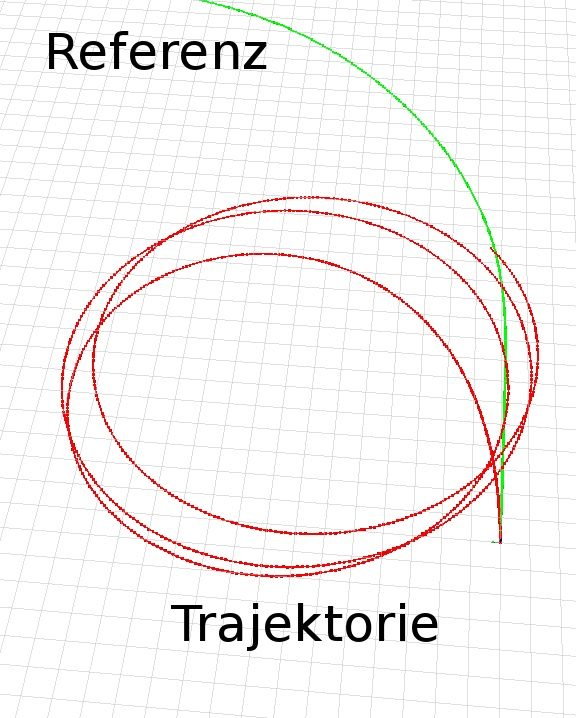
\includegraphics[width=0.5\textwidth]{Ergebnis_Failed}
\caption{Ergebnis Failedx}
\label{fig:Ergebnis_Failed}
\end{center}
\end{figure} 

\subsection{Lenkung} %(fold)
Die Feature-Raum hat eine unzureichende Abdeckung mit Lerndaten und deswegen die schlechte Generalisierung. Siehe Abbildung ~\ref{fig:Ergebnis_NN-winkel}.

\begin{figure}[htbp]
\begin{center}
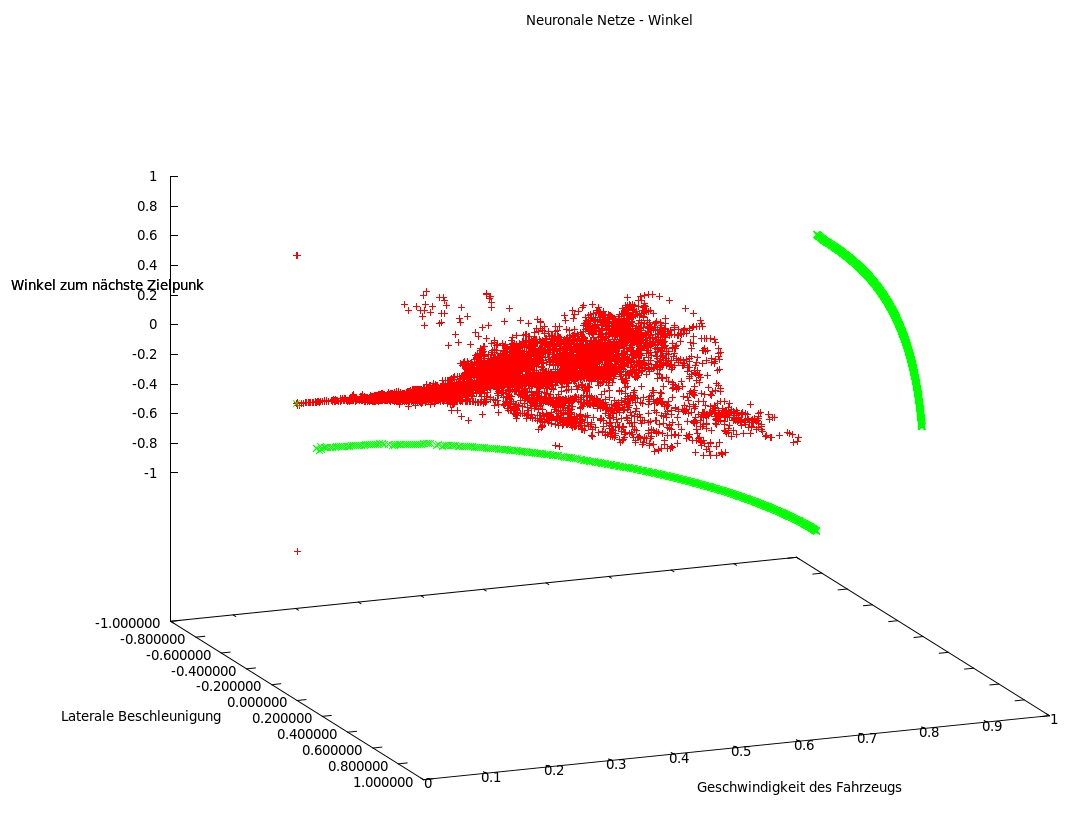
\includegraphics[width=0.8\textwidth]{Ergebnis_NN-winkel}
\caption{Ergebnis NN-winkel}
\label{fig:Ergebnis_NN-winkel}
\end{center}
\end{figure}
% subsection Lenkung (end)

\subsection{Gaspedal} %(fold)
Die Feature-Raum hat eine unzureichende Abdeckung mit Lerndaten und deswegen die schlechte Generalisierung. Siehe Abbildung ~\ref{fig:Ergebnis_SVM-gas}.

\begin{figure}[htbp]
\begin{center}
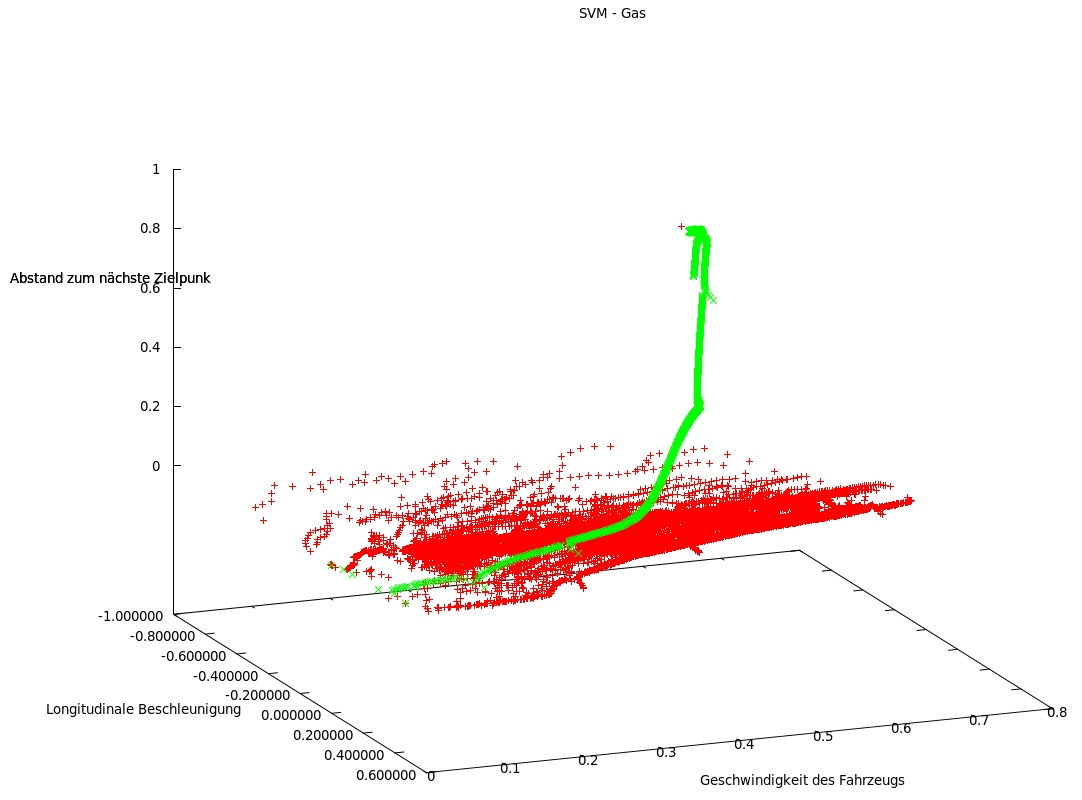
\includegraphics[width=0.8\textwidth]{Ergebnis_SVM-gas}
\caption{Ergebnis SVM-gas}
\label{fig:Ergebnis_SVM-gas}
\end{center}
\end{figure}
% subsection Lenkung (end)

% section Online (end)


\section{Offline} % (fold)
\label{sec:Offline}
Die Evaluation oder Vergleich zwischen die verschiedene Verfahren wurde Offline gemacht, da alle bei Online-Tests Problemen hatten. Die Evaluation besteht aus die Abgleich der Ist- und Sollwerte (Siehe Abbildung ~\ref{fig:Ergebnis_x}). Die Eingaben sind die Feature-Vektoren (Referenz) und die Ausgaben sind die Stellgrößen (Lernverfahren). Danach eine Graphik mit Stellgröße (Referenz) zu Stellgröße (Lernverfahren) wurde für jeder Verfahren gemacht (Siehe Abbildung ~\ref{fig:Ergebnis_Evaluation}). Dieses Szenario hat sehr gute Performance gezeigt.

\begin{figure}[htbp]
\begin{center}
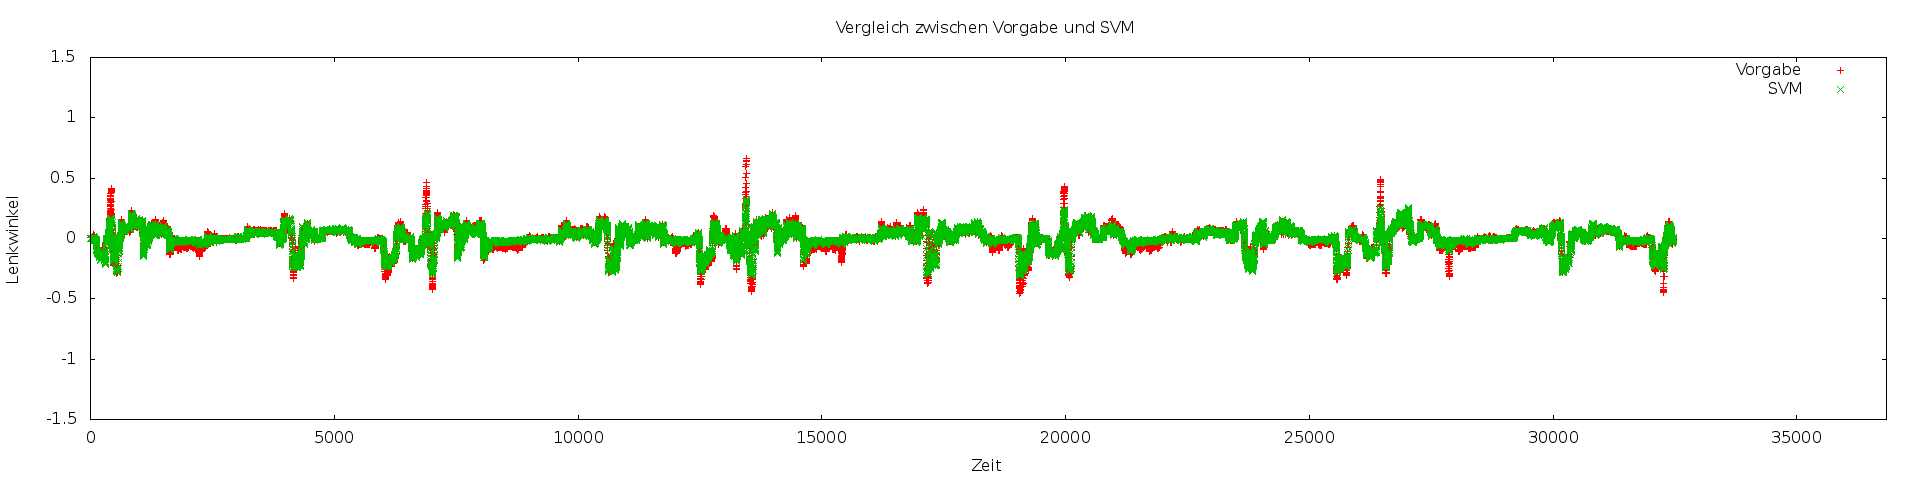
\includegraphics[width=0.9\textwidth]{Ergebnis_x}
\caption{Evaluation: Vergleich zwischen Soll- und Istwerten}
\label{fig:Ergebnis_x}
\end{center}
\end{figure}

\begin{figure}[htbp]
\begin{center}
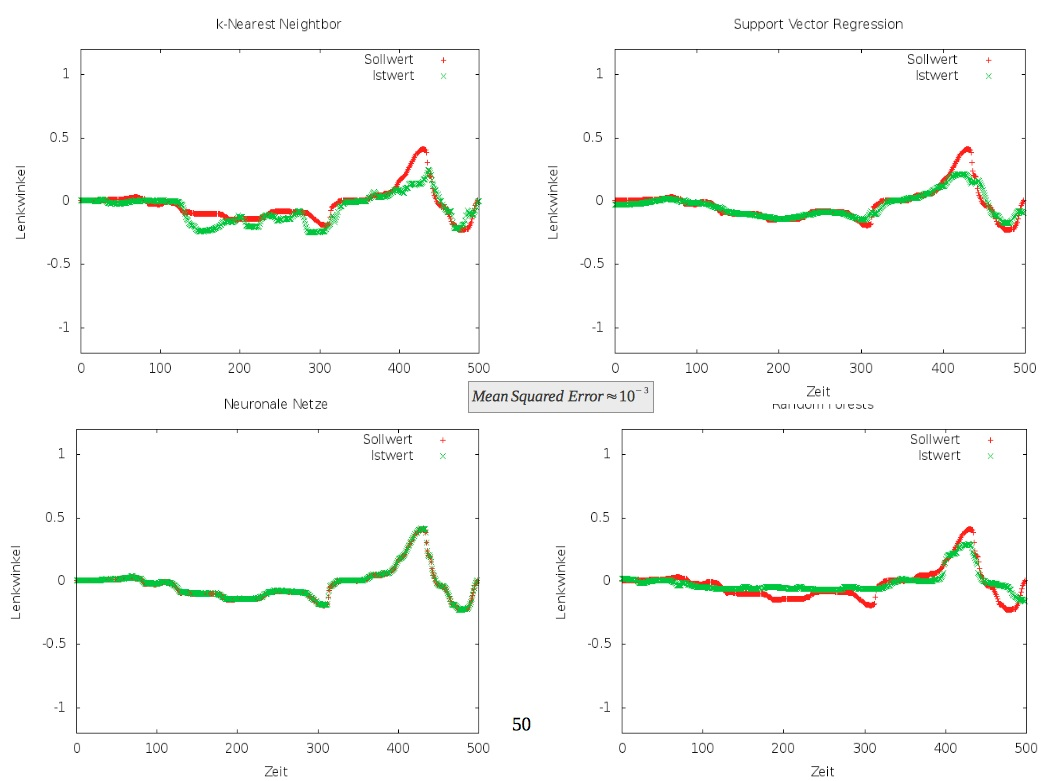
\includegraphics[width=1\textwidth]{Ergebnis_Evaluation}
\caption{Ergebnis Evaluation mit die Verfahren}
\label{fig:Ergebnis_Evaluation}
\end{center}
\end{figure}
% section Offline (end)


% chapter Ergebnise (end)
